\documentclass{standalone}
\usepackage{tikz}
\usetikzlibrary{patterns, positioning}


\begin{document}
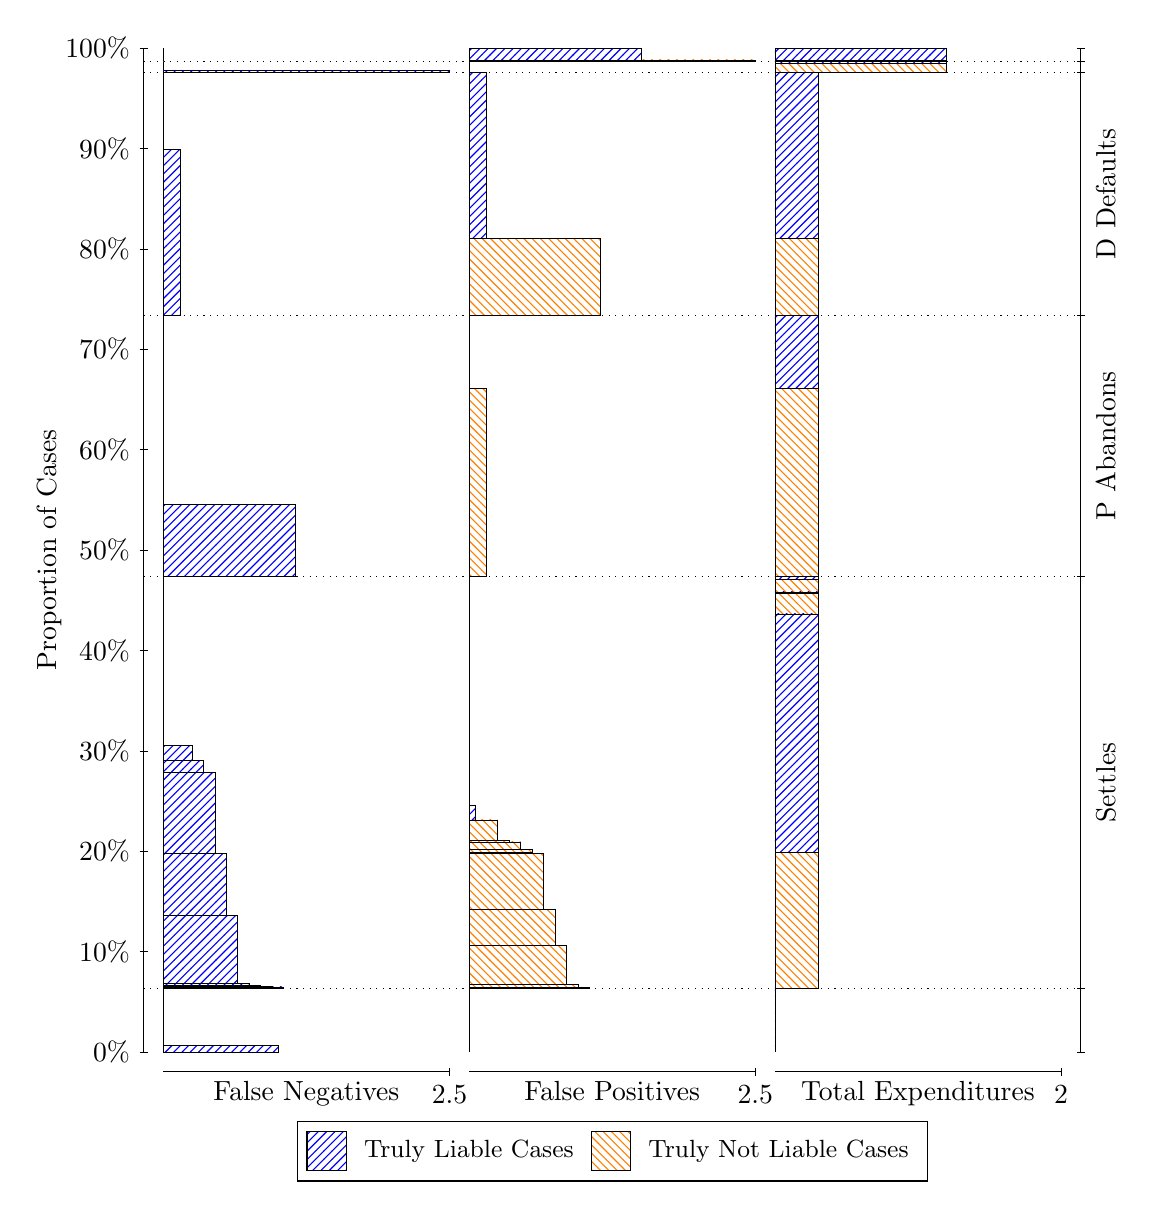
\begin{tikzpicture}
\draw[black, very thin] (1.5,1.75) -- (1.5,14.5);
\node[rotate=90, text=black, anchor=center] at (0.3, 8.125) {Proportion of Cases};
\draw[black, very thin] (1.45,1.75) -- (1.55,1.75);
\node[text=black, anchor=east] at (1.45, 1.75) {0\%};
\draw[black, very thin] (1.45,3.025) -- (1.55,3.025);
\node[text=black, anchor=east] at (1.45, 3.025) {10\%};
\draw[black, very thin] (1.45,4.3) -- (1.55,4.3);
\node[text=black, anchor=east] at (1.45, 4.3) {20\%};
\draw[black, very thin] (1.45,5.575) -- (1.55,5.575);
\node[text=black, anchor=east] at (1.45, 5.575) {30\%};
\draw[black, very thin] (1.45,6.85) -- (1.55,6.85);
\node[text=black, anchor=east] at (1.45, 6.85) {40\%};
\draw[black, very thin] (1.45,8.125) -- (1.55,8.125);
\node[text=black, anchor=east] at (1.45, 8.125) {50\%};
\draw[black, very thin] (1.45,9.4) -- (1.55,9.4);
\node[text=black, anchor=east] at (1.45, 9.4) {60\%};
\draw[black, very thin] (1.45,10.675) -- (1.55,10.675);
\node[text=black, anchor=east] at (1.45, 10.675) {70\%};
\draw[black, very thin] (1.45,11.95) -- (1.55,11.95);
\node[text=black, anchor=east] at (1.45, 11.95) {80\%};
\draw[black, very thin] (1.45,13.225) -- (1.55,13.225);
\node[text=black, anchor=east] at (1.45, 13.225) {90\%};
\draw[black, very thin] (1.45,14.5) -- (1.55,14.5);
\node[text=black, anchor=east] at (1.45, 14.5) {100\%};

\draw[black, very thin] (13.4,1.75) -- (13.4,14.5);
\draw[black, very thin] (13.35,1.75) -- (13.45,1.75);
\node[anchor=west] at (13.35, 1.75) {};
\draw[black, very thin] (13.35,2.5554) -- (13.45,2.5554);
\node[anchor=west] at (13.35, 2.5554) {};
\draw[black, very thin] (13.35,7.7854) -- (13.45,7.7854);
\node[anchor=west] at (13.35, 7.7854) {};
\draw[black, very thin] (13.35,11.103) -- (13.45,11.103);
\node[anchor=west] at (13.35, 11.103) {};
\draw[black, very thin] (13.35,14.193) -- (13.45,14.193);
\node[anchor=west] at (13.35, 14.193) {};
\draw[black, very thin] (13.35,14.329) -- (13.45,14.329);
\node[anchor=west] at (13.35, 14.329) {};
\draw[black, very thin] (13.35,14.5) -- (13.45,14.5);
\node[anchor=west] at (13.35, 14.5) {};

\draw[black, very thin, pattern color=blue, pattern=north east lines] (1.75,1.75) rectangle (3.2033,1.8347);
\draw[black, very thin, pattern color=orange, pattern=north west lines] (1.75,1.8347) rectangle (1.75,2.5554);
\draw[black, very thin, pattern color=blue, pattern=north east lines] (1.75,2.5554) rectangle (3.276,2.5769);
\draw[black, very thin, pattern color=blue, pattern=north east lines] (1.75,2.5769) rectangle (3.1307,2.5787);
\draw[black, very thin, pattern color=blue, pattern=north east lines] (1.75,2.5787) rectangle (2.9853,2.5988);
\draw[black, very thin, pattern color=blue, pattern=north east lines] (1.75,2.5988) rectangle (2.84,2.62);
\draw[black, very thin, pattern color=blue, pattern=north east lines] (1.75,2.62) rectangle (2.6947,3.4876);
\draw[black, very thin, pattern color=blue, pattern=north east lines] (1.75,3.4876) rectangle (2.5493,4.2707);
\draw[black, very thin, pattern color=blue, pattern=north east lines] (1.75,4.2707) rectangle (2.404,5.2959);
\draw[black, very thin, pattern color=blue, pattern=north east lines] (1.75,5.2959) rectangle (2.2587,5.4547);
\draw[black, very thin, pattern color=blue, pattern=north east lines] (1.75,5.4547) rectangle (2.1133,5.642);
\draw[black, very thin, pattern color=orange, pattern=north west lines] (1.75,5.642) rectangle (1.75,7.7854);
\draw[black, very thin, pattern color=blue, pattern=north east lines] (1.75,7.7854) rectangle (3.4213,8.7062);
\draw[black, very thin, pattern color=orange, pattern=north west lines] (1.75,8.7062) rectangle (1.75,11.103);
\draw[black, very thin, pattern color=blue, pattern=north east lines] (1.75,11.103) rectangle (1.968,13.215);
\draw[black, very thin, pattern color=orange, pattern=north west lines] (1.75,13.215) rectangle (1.75,14.193);
\draw[black, very thin, pattern color=blue, pattern=north east lines] (1.75,14.193) rectangle (5.3833,14.213);
\draw[black, very thin, pattern color=orange, pattern=north west lines] (1.75,14.213) rectangle (1.75,14.329);
\draw[black, very thin, pattern color=orange, pattern=north west lines] (1.75,14.329) rectangle (1.75,14.349);
\draw[black, very thin, pattern color=blue, pattern=north east lines] (1.75,14.349) rectangle (1.75,14.5);
\draw[black, very thin, pattern color=orange, pattern=north west lines] (5.6333,1.75) rectangle (5.6333,2.4706);
\draw[black, very thin, pattern color=blue, pattern=north east lines] (5.6333,2.4706) rectangle (5.6333,2.5554);
\draw[black, very thin, pattern color=orange, pattern=north west lines] (5.6333,2.5554) rectangle (7.1593,2.5689);
\draw[black, very thin, pattern color=orange, pattern=north west lines] (5.6333,2.5689) rectangle (7.014,2.6036);
\draw[black, very thin, pattern color=orange, pattern=north west lines] (5.6333,2.6036) rectangle (6.8687,3.1038);
\draw[black, very thin, pattern color=orange, pattern=north west lines] (5.6333,3.1038) rectangle (6.7233,3.5588);
\draw[black, very thin, pattern color=orange, pattern=north west lines] (5.6333,3.5588) rectangle (6.578,4.2727);
\draw[black, very thin, pattern color=orange, pattern=north west lines] (5.6333,4.2727) rectangle (6.4327,4.2839);
\draw[black, very thin, pattern color=orange, pattern=north west lines] (5.6333,4.2839) rectangle (6.4327,4.326);
\draw[black, very thin, pattern color=orange, pattern=north west lines] (5.6333,4.326) rectangle (6.2873,4.4177);
\draw[black, very thin, pattern color=orange, pattern=north west lines] (5.6333,4.4177) rectangle (6.142,4.4393);
\draw[black, very thin, pattern color=orange, pattern=north west lines] (5.6333,4.4393) rectangle (5.9967,4.6988);
\draw[black, very thin, pattern color=blue, pattern=north east lines] (5.6333,4.6988) rectangle (5.706,4.8861);
\draw[black, very thin, pattern color=blue, pattern=north east lines] (5.6333,4.8861) rectangle (5.6333,7.7854);
\draw[black, very thin, pattern color=orange, pattern=north west lines] (5.6333,7.7854) rectangle (5.8513,10.182);
\draw[black, very thin, pattern color=blue, pattern=north east lines] (5.6333,10.182) rectangle (5.6333,11.103);
\draw[black, very thin, pattern color=orange, pattern=north west lines] (5.6333,11.103) rectangle (7.3047,12.08);
\draw[black, very thin, pattern color=blue, pattern=north east lines] (5.6333,12.08) rectangle (5.8513,14.193);
\draw[black, very thin, pattern color=orange, pattern=north west lines] (5.6333,14.193) rectangle (5.6333,14.309);
\draw[black, very thin, pattern color=blue, pattern=north east lines] (5.6333,14.309) rectangle (5.6333,14.329);
\draw[black, very thin, pattern color=orange, pattern=north west lines] (5.6333,14.329) rectangle (9.2667,14.349);
\draw[black, very thin, pattern color=blue, pattern=north east lines] (5.6333,14.349) rectangle (7.8133,14.5);
\draw[black, very thin, pattern color=orange, pattern=north west lines] (9.5167,1.75) rectangle (9.5167,2.4706);
\draw[black, very thin, pattern color=blue, pattern=north east lines] (9.5167,2.4706) rectangle (9.5167,2.5554);
\draw[black, very thin, pattern color=orange, pattern=north west lines] (9.5167,2.5554) rectangle (10.062,4.2839);
\draw[black, very thin, pattern color=blue, pattern=north east lines] (9.5167,4.2839) rectangle (10.062,7.3126);
\draw[black, very thin, pattern color=orange, pattern=north west lines] (9.5167,7.3126) rectangle (10.062,7.572);
\draw[black, very thin, pattern color=blue, pattern=north east lines] (9.5167,7.572) rectangle (10.062,7.5936);
\draw[black, very thin, pattern color=orange, pattern=north west lines] (9.5167,7.5936) rectangle (10.062,7.749);
\draw[black, very thin, pattern color=blue, pattern=north east lines] (9.5167,7.749) rectangle (10.062,7.7854);
\draw[black, very thin, pattern color=orange, pattern=north west lines] (9.5167,7.7854) rectangle (10.062,10.182);
\draw[black, very thin, pattern color=blue, pattern=north east lines] (9.5167,10.182) rectangle (10.062,11.103);
\draw[black, very thin, pattern color=orange, pattern=north west lines] (9.5167,11.103) rectangle (10.062,12.08);
\draw[black, very thin, pattern color=blue, pattern=north east lines] (9.5167,12.08) rectangle (10.062,14.193);
\draw[black, very thin, pattern color=orange, pattern=north west lines] (9.5167,14.193) rectangle (11.697,14.309);
\draw[black, very thin, pattern color=blue, pattern=north east lines] (9.5167,14.309) rectangle (11.697,14.329);
\draw[black, very thin, pattern color=orange, pattern=north west lines] (9.5167,14.329) rectangle (11.697,14.349);
\draw[black, very thin, pattern color=blue, pattern=north east lines] (9.5167,14.349) rectangle (11.697,14.5);
\draw[black, dotted] (1.5,2.5554) -- (13.4,2.5554);
\draw[black, dotted] (1.5,7.7854) -- (13.4,7.7854);
\draw[black, dotted] (1.5,11.103) -- (13.4,11.103);
\draw[black, dotted] (1.5,14.193) -- (13.4,14.193);
\draw[black, dotted] (1.5,14.329) -- (13.4,14.329);
\draw[black, very thin] (1.75,1.5) -- (5.3833,1.5);
\node[text=black, anchor=north] at (3.5667, 1.5) {False Negatives};
\draw[black, very thin] (5.3833,1.45) -- (5.3833,1.55);
\node[text=black, anchor=north] at (5.3833, 1.45) {2.5};

\draw[black, very thin] (5.6333,1.5) -- (9.2667,1.5);
\node[text=black, anchor=north] at (7.45, 1.5) {False Positives};
\draw[black, very thin] (9.2667,1.45) -- (9.2667,1.55);
\node[text=black, anchor=north] at (9.2667, 1.45) {2.5};

\draw[black, very thin] (9.5167,1.5) -- (13.15,1.5);
\node[text=black, anchor=north] at (11.333, 1.5) {Total Expenditures};
\draw[black, very thin] (13.15,1.45) -- (13.15,1.55);
\node[text=black, anchor=north] at (13.15, 1.45) {2};


\node[text=black, centered, rotate=90] at (13.72, 5.1704) {Settles};
\node[text=black, centered, rotate=90] at (13.72, 9.4443) {P Abandons};
\node[text=black, centered, rotate=90] at (13.72, 12.648) {D Defaults};



\draw (7.449999999999999,1.5) node[draw=none] (baseCoordinate) {};
\begin{scope}[align=center]
        \matrix[scale=0.5, draw=black, below=0.5cm of baseCoordinate, nodes={draw}, column sep=0.1cm]{
            \node[rectangle, draw, minimum width=0.5cm, minimum height=0.5cm, pattern color=blue, pattern=north east lines] {}; &
            \node[draw=none, font=\small, text=black] (B) {Truly Liable Cases}; &
            \node[rectangle, draw, minimum width=0.5cm, minimum height=0.5cm, pattern color=orange, pattern=north west lines] {}; &
            \node[draw=none, font=\small, text=black] (B) {Truly Not Liable Cases}; \\
            };
\end{scope}

\end{tikzpicture}
\end{document}